\documentclass[8pt,a4paper,compress]{beamer}

\usepackage{/home/siyer/lib/slides}

\title{Input and Output (IO), Objects, and Plotting with Matplotlib}
\date{}

\begin{document}
\begin{frame}
\vfill
\titlepage
\end{frame}

\begin{frame}
\frametitle{Outline}
\tableofcontents
\end{frame}

\section{Standard Output}
\begin{frame}[fragile]
\begin{center}
\begin{tikzpicture}
\begin{scope}[->,xshift=-7.5cm,yshift=-5cm,thin,
	   node distance=1.6cm,on grid,>=stealth,
  	   block1/.style={rectangle,draw,align=center},
	   block2/.style={rectangle,align=center}]
\node [block2] (1) {input};
\node [block1] (2) [right=of 1] {\lstinline$my_program.py$};
\node [block2] (3) [right=of 2] {output};
\path (1) edge node [above] {} (2);
\path (2) edge node [above] {} (3);
\end{scope}
\end{tikzpicture}
\end{center}

\bigskip

Input
\begin{itemize}
\item Command-line input: The mechanism we have been using to provide
input values to our programs. We list them after the program name and access them using the \lstinline{sys.argv} list within the program
\item Standard input: Makes it possible to write programs that
process arbitrary amounts of input and to interact with the programs
\end{itemize}

\bigskip

Output
\begin{itemize}
\item Standard output: The mechanism we have been using to print output from our programs to the terminal window. We use methods such as \lstinline{stdio.write()} and \lstinline{stdio.writeln()}
\item Standard drawing: Makes it possible to work with graphical representations of images
\end{itemize}
\end{frame}

\begin{frame}[fragile]
\begin{framed}
\tiny randomseq.py: Accept an integer command-line argument $n$. Write to standard output a random sequence of $n$ floats in the range $[0, 1)$.
\end{framed}

\begin{lstlisting}[language=Python]
import random
import stdio
import sys

n = int(sys.argv[1])
for i in range(n):
    stdio.writeln(random.random())
\end{lstlisting}

\begin{lstlisting}[language={}]
$ python randomseq.py 10
0.534835410847
0.249397020334
0.0460440369486
0.608142728098
0.686734322334
0.508728644023
0.831805280108
0.474190147291
0.89541446225
0.671581101113
\end{lstlisting}
\end{frame}

\begin{frame}[fragile]
API for the \lstinline{stdio} module relevant to standard output
\begin{center}
\begin{tabular}{cc}
function & description \\ \hline
\lstinline$stdio.write(x)$ & write $x$ to standard output \\
\lstinline$stdio.writeln(x)$ & write $x$ to standard output, followed by a newline \\
\lstinline$stdio.writef(fmt, arg1, ...)$ & \makecell{write the arguments $arg_1, \dots$ to standard output \\ as specified by the format string $fmt$} \\
\end{tabular} 
\end{center}

\bigskip

Formatted writing: In its simplest form, \lstinline{stdio.writef()} takes two arguments; The first argument is a format string that describes how to convert the second argument into a string for output;  For example
\begin{lstlisting}[language=Python]
stdio.writef('pi is approximately %.2f.\n', math.pi)
\end{lstlisting}
writes the output
\begin{lstlisting}[language={}]
pi is approximately 3.14.
\end{lstlisting}

\bigskip

The \lstinline{stdio.writef()} function can take more than two arguments, in which case, the format string will have a format specifier for each additional argument, perhaps separated by other characters to pass through to the output; For example
\begin{lstlisting}[language=Python]
stdio.writef('The %dth decimal digit of %.10f is %d.\n', 5, math.pi, 9)
\end{lstlisting}
writes the output
\begin{lstlisting}[language={}]
The 5th decimal digit of 3.1415926536 is 9.
\end{lstlisting}
\end{frame}

\section{Standard Input}
\begin{frame}[fragile]
The \emph{standard input stream} is an abstract data stream that may be empty or may contain a sequence of values separated by whitespace 

\bigskip

The end of the input stream is marked by the end-of-file (EOF) character, specified using \lstinline$<ctrl-d>$ or \lstinline$<ctrl-z>$ 

\bigskip

The \lstinline{stdio} module also supports reading from standard input stream

\bigskip

A program that reads from standard input stream consumes the values, ie, it cannot back up and read them again
\end{frame}

\begin{frame}[fragile]
API for the \lstinline$stdio$ module relevant to standard input
\begin{center}
\begin{tabular}{cc}
function & description \\ \hline
\lstinline$stdio.isEmpty()$ & is the standard input empty (or only whitespace)? \\
\lstinline$stdio.readInt()$ & read a token, convert it to an integer, and return it \\
\lstinline$stdio.readFloat()$ & read a token, convert it to a float, and return it \\
\lstinline$stdio.readBool()$ & read a token, convert it to a boolean, and return it \\
\lstinline$stdio.readString()$ & read a token and return it as a string \\
\lstinline$stdio.hasNextLine()$ & does standard input have a next line? \\
\lstinline$stdio.readLine()$ & read the next line and return it as a string \\
\lstinline$stdio.readAll()$ & read all remaining input and return it as a string \\
\lstinline$stdio.readAllInts()$ & read all remaining tokens and return them as a list of integers \\
\lstinline$stdio.readAllFloats()$ & read all remaining tokens and return them as a list of floats \\
\lstinline$stdio.readAllBools()$ & read all remaining tokens and return them as a list of booleans \\
\lstinline$stdio.readAllStrings()$ & read all remaining tokens and return them as a list of strings \\
\lstinline$stdio.readAllLines()$ & read all remaining lines and return them as a list of strings
\end{tabular} 
\end{center}
\end{frame}

\begin{frame}[fragile]
\begin{framed}
\tiny average.py: Read floats from the standard input stream until end-of-file. Write to standard output the average of those floats.
\end{framed}

\begin{lstlisting}[language=Python]
import stdio

total = 0.0
count = 0
while not stdio.isEmpty():
    value = stdio.readFloat()
    total += value
    count += 1
avg = total / count
stdio.writeln('Average is ' + str(avg))
\end{lstlisting}

\begin{lstlisting}[language={}]
$ python average.py
10.0 5.0 6.0
3.0
7.0 32.0
<ctrl-d>
Average is 10.5
\end{lstlisting}
\end{frame}

\section{Redirection and Piping}
\begin{frame}[fragile]
By adding the directive \lstinline{>} to the command that invokes a program, we can redirect its standard output to a file, either for permanent storage or for input to another program at a later time; For example
\begin{lstlisting}[language={}]
$ python randomseq.py 1000 > data.txt
$ head -5 data.txt 
0.12490675039
0.509198876091
0.224604151916
0.918194898729
0.296035502122
\end{lstlisting}

\bigskip

Similarly, by adding the directive \lstinline{<} to the command that invokes a program, we can redirect standard input so that \lstinline{stdio} reads data from a file instead of the terminal; For example
\begin{lstlisting}[language={}]
$ python average.py < data.txt
Average is 0.499379975213
\end{lstlisting}

\bigskip

The standard output of one program can be mapped to the standard input stream of another program using the (pipe) directive \lstinline{|}; For example
\begin{lstlisting}[language={}]
$ python randomseq.py 1000 | python average.py 
Average is 0.501346917807
$ python randomseq.py 1000 | python average.py | wc
      1       3      26
\end{lstlisting}
\end{frame}

\section{Methods}
\begin{frame}[fragile]
A \emph{method} is a function associated with a specific object (and, by extension, with the type of that object)

\bigskip

We \emph{call} (or \emph{invoke}) a method using a variable name, followed by the dot operator (\lstinline{.}), followed by the method name, followed by its arguments separated by commas and enclosed in parentheses

\begin{lstlisting}[language={}]
x = 3 ** 100
bits = x.bit_length()
stdio.writeln(bits)
\end{lstlisting}

\bigskip

Methods in the built-in \lstinline{str} data type
\begin{lstlisting}[language={}]
>>> dir(str)
[..., 'capitalize', 'center', 'count', 'decode', 'encode', 'endswith', 
'expandtabs', 'find', 'format', 'index', 'isalnum', 'isalpha', 'isdigit', 
'islower', 'isspace', 'istitle', 'isupper', 'join', 'ljust', 'lower', 'lstrip', 
'partition', 'replace', 'rfind', 'rindex', 'rjust', 'rpartition', 'rsplit', 
'rstrip', 'split', 'splitlines', 'startswith', 'strip', 'swapcase', 'title', 
'translate', 'upper', 'zfill']
\end{lstlisting}
\end{frame}

\begin{frame}[fragile]
\begin{framed}
\tiny potentialgene.py: Accepts a DNA sequence as a command-line argument, and writes \lstinline{True} to standard output if the sequence corresponds to a potential gene, and \lstinline{False} otherwise.
\end{framed}

\begin{lstlisting}[language=Python]
import stdio
import sys

def isPotentialGene(dna):
    if (len(dna) % 3) != 0: return False
    if not dna.startswith('ATG'): return False
    for i in range(len(dna) - 3):
        if i % 3 == 0:
            if dna[i:i + 3] == 'TAA': return False
            if dna[i:i + 3] == 'TAG': return False
            if dna[i:i + 3] == 'TGA': return False
    if dna.endswith('TAA'): return True
    if dna.endswith('TAG'): return True
    if dna.endswith('TGA'): return True
    return False

def main():
    dna = sys.argv[1]
    stdio.writeln(isPotentialGene(dna))

if __name__ == '__main__':
    main()
\end{lstlisting}

\begin{lstlisting}[language={}]
$ python potentialgene.py ATGCGCCTGCGTCTGTACTAG
True
$ python potentialgene.py ATGCGCTGCGTCTGTACTAG
False
\end{lstlisting}
\end{frame}

\section{Plotting with Matplotlib}
\begin{frame}[fragile]
The most important function in Matplotlib, a third-party plotting library, is \lstinline{plot()}, which allows us to plot 2D data

\begin{minipage}{150pt}
\begin{lstlisting}[language=Python]
import numpy as np
import matplotlib.pyplot as plt

x = np.arange(0, 3 * np.pi, 0.1)
y = np.sin(x)
plt.plot(x, y)
plt.show()
\end{lstlisting}
\end{minipage}%
\begin{minipage}{150pt}
\begin{center}
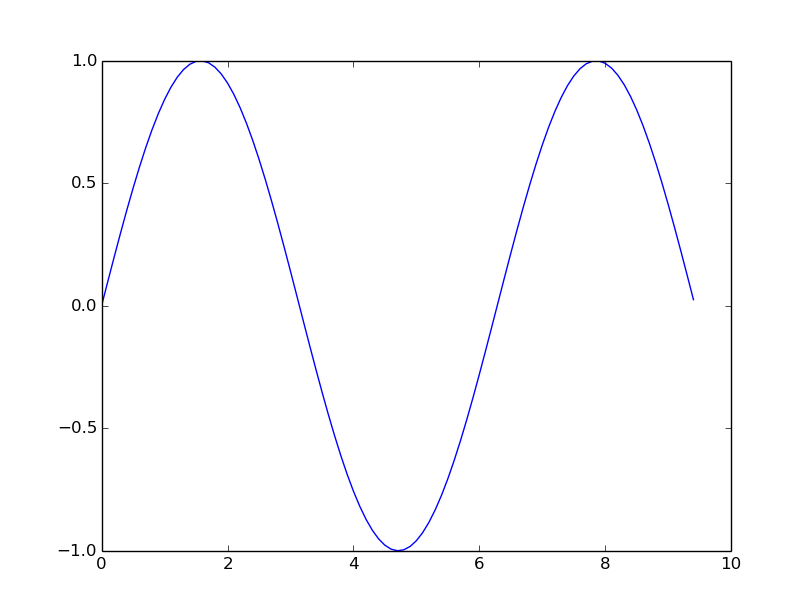
\includegraphics[scale=0.2]{figures/sin.png}

\smallskip

\lstinline{$ python sin.py}
\end{center}
\end{minipage}

\bigskip

We can plot multiple lines at once, add a title, legend, and axis labels

\begin{minipage}{150pt}
\begin{lstlisting}[language=Python]
import numpy as np
import matplotlib.pyplot as plt

x = np.arange(0, 3 * np.pi, 0.1)
y_sin = np.sin(x)
y_cos = np.cos(x)
plt.plot(x, y_sin)
plt.plot(x, y_cos)
plt.xlabel('x axis label')
plt.ylabel('y axis label')
plt.title('Sine and Cosine')
plt.legend(['Sine', 'Cosine'])
plt.show()
\end{lstlisting}
\end{minipage}%
\begin{minipage}{150pt}
\begin{center}
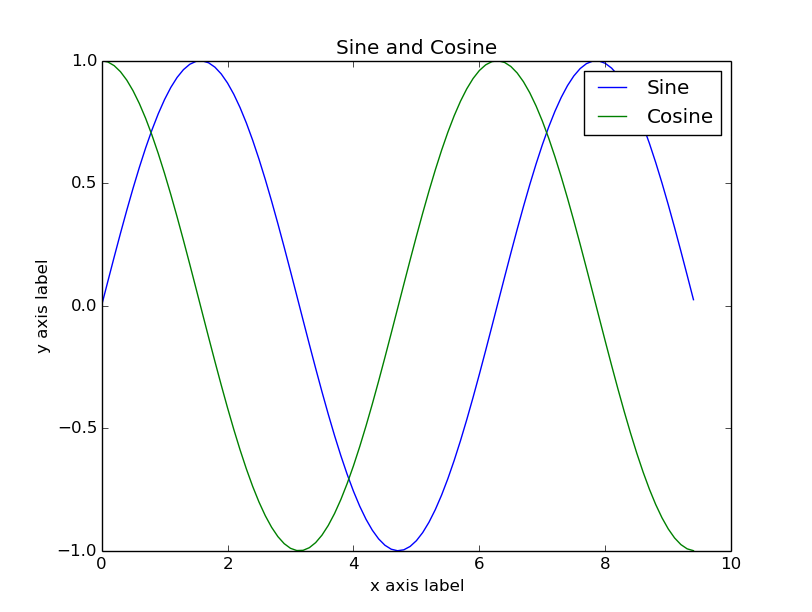
\includegraphics[scale=0.2]{figures/sin_cos.png}

\smallskip

\lstinline{$ python sin_cos.py}
\end{center}
\end{minipage}
\end{frame}

\begin{frame}[fragile]
We can also save the plot to a file

\begin{minipage}{200pt}
\begin{lstlisting}[language=Python]
import matplotlib.pyplot as plt
import stdio

lines = stdio.readAllLines()
x = []
y = []
for line in lines:
    toks = line.strip().split(',')
    x.append(int(toks[0]))
    y.append(float(toks[1]))
plt.plot(x, y)
plt.title('Wolf\'s Sunspot Numbers (1700 - 1988)')
plt.xlabel('Year')
plt.ylabel('Number of sunspots')
plt.savefig('sunspots.png')
\end{lstlisting}

\begin{lstlisting}[language={}]
$ head -5 sunspots.csv
1700,5.0
1701,11.0
1702,16.0
1703,23.0
1704,36.0
...
\end{lstlisting}
\end{minipage}%
\begin{minipage}{100pt}
\begin{center}
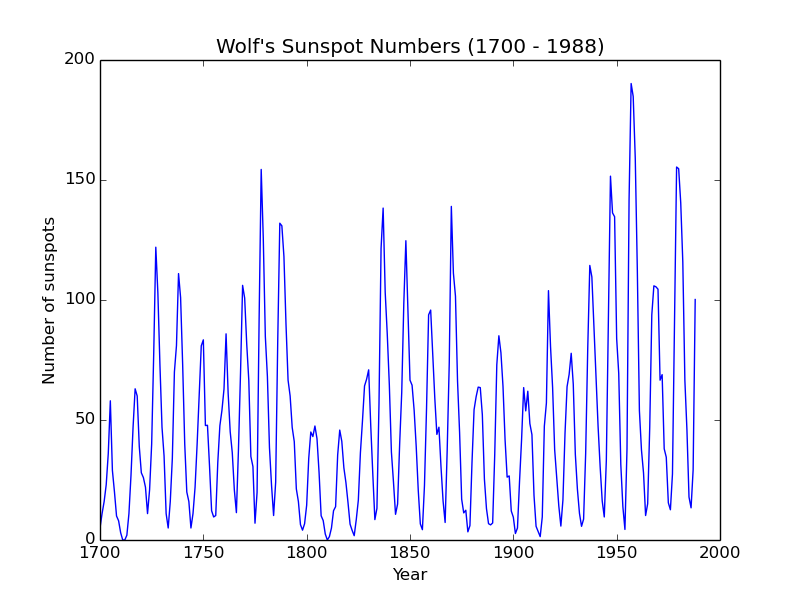
\includegraphics[scale=0.2]{figures/sunspots.png}

\smallskip

\lstinline{$ python sunspots.py < sunspots.txt}
\end{center}
\end{minipage}
\end{frame}

\section{Exercises}
\begin{frame}[fragile]
\begin{enumerate}
\item Write a program \lstinline{min_max.py} that reads in floats (as many as the user enters) from standard input and writes out the minimum and maximum values along with their ranks, ie, their positions (starting at 1) in the input.

\begin{lstlisting}[language={}]
$ python min_max.py
3.0 1.0 5.0 4.0 2.0
<ctrl-d>
min val = 1.000000, min rank = 2
max val = 5.000000, max rank = 3
\end{lstlisting}

\item Write a program  \lstinline{means.py} that reads in positive real numbers from standard input and writes their geometric and harmonic means. The \emph{geome
tric mean} of $n$ positive numbers $x_1, x_2, \dots, x_n$ is $(x_1 \times x_2 \times \cdots \times x_n)^{1/n}$ and their \emph{harmonic mean} is $n / (1/x_1 + 1/x_2 + \cdots + 1/x_n)$. Hint: for the geometric mean, consider taking logarithms to avoid overflow.

\begin{lstlisting}[language={}]
$ python means.py
1.0 2.0 3.0 4.0 5.0
<ctrl-d>
geometric mean = 2.605171, harmonic mean = 2.189781
\end{lstlisting}
\end{enumerate}
\end{frame}

\begin{frame}[fragile]
\begin{enumerate}\setcounter{enumi}{2}
\item Write a program that takes three floats $x$, $y$, and $z$ from the command line, reads from standard input a sequence of coordinates $(x_i, y_i, z_i)$, and writes the coordinates of the point closest to $(x, y, z)$. Recall that the square of the distance between $(x, y, z)$ and $(x_i, y_i, z_i)$ is $(x-x_i)^2+(y-y_i)^2+(z-z_i)^2$. For efficiency, do not use either \lstinline{math.sqrt()} or the \lstinline{**} operator.

\begin{lstlisting}[language={}]
$ python closest.py 1.0 5.0 2.0
1.0 3.0 9.0 5.0 3.0 2.5 9.0 6.0 2.0 2.0 6.0 3.0 5.0 6.0 5.0
<ctrl-d>
closest point = (2.000000, 6.000000, 3.000000)
\end{lstlisting}

\item  Implement the function \lstinline{is_valid()} in \lstinline{password_checker.py} that returns \lstinline{True} if the given password string meets the following specific
ations, and \lstinline{False} otherwise:
\begin{itemize}
\item At least eight characters long.
\item Contains at least one digit (0-9).
\item Contains at least one uppercase letter.
\item Contains at least one lowercase letter.
\item Contains at least one character that is neither a letter nor a number.
\end{itemize}
\begin{lstlisting}
$ python password_checker.py Abcde1fg
False
$ python password_checker.py Abcde1@g
True
\end{lstlisting} 
\end{enumerate}
\end{frame}


\begin{frame}[fragile]
\begin{enumerate}\setcounter{enumi}{4}
\item The \emph{Jaccard index} measures the similarity between finite sample sets, and is defined as the size of the intersection divided by the size of the union of the sample sets: $$J(A, B) = \frac{|A\cap B|}{|A\cup B|}.$$ Note that $0 \leq J(A, B) \leq 1$. The \emph{Jaccard distance}, which measures dissimilarity between sample sets, is complementary to the Jaccard index and is obtained by subtracting the Jaccard index from 1: $$d_J(A, B)=1-J(A, B).$$

\noindent Implement the functions \lstinline{jaccard_index()} and \lstinline{jaccard_distance()} in \lstinline{set_distance.py} that take two sets $A$ and $B$ as arguments and return their Jaccard index and J
accard distance, respectively.

\begin{lstlisting}
$ python set_distance.py "b, c" "a, b, c, d"
0.5
$ python set_distance.py "7, 3, 2, 4, 1" "4, 1, 9, 7, 5"
0.571428571429
\end{lstlisting} 
\end{enumerate}
\end{frame}
\end{document}
